\documentclass[10pt,oneside]{article}

\usepackage{amsmath}
\usepackage{amssymb} % for \checkmark
\usepackage{bm}
\usepackage{mathpazo}
\usepackage{graphicx}
\usepackage{enumerate}
\usepackage[x11names, svgnames]{xcolor} % for \definecolor

\usepackage[letterpaper]{geometry}
\geometry{verbose,tmargin=0.25in,bmargin=0.5in,lmargin=1in,rmargin=1.15in}

 \definecolor{saitPurple}{RGB}{112,40,119}
 \definecolor{statsMaroon}{rgb}{0.55, 0, 0}
 \definecolor{saitMaroon}{rgb}{0.55, 0, 0}
 \definecolor{statsRed}{RGB}{224,38,37}
 \definecolor{saitRed}{RGB}{224,38,37}
 \definecolor{saitBlue}{rgb}{0, 0.59, 0.85}
 \definecolor{statsBlue}{rgb}{0, 0.59, 0.85}
 \definecolor{statsDeepBlue}{RGB}{0, 99, 167}
 \definecolor{saitDeepBlue}{RGB}{0, 99, 167}
 \definecolor{saitDeepBlue}{RGB}{0, 99, 167}
 \definecolor{LightGrey}{RGB}{200,200,200}
%  \definecolor{boxBG}{RGB}{236, 227, 227}
%  \definecolor{boxBG}{RGB}{242, 233, 223}
\usepackage{xcolor}
\usepackage{cancel}
\usepackage{bm}
\usepackage{graphicx}
\usepackage[x11names, svgnames]{xcolor} % for colors in handouts, auto loaded in Beamer?
\usepackage{tikz}
\usetikzlibrary{arrows.meta, math, calc, shadows}
\usetikzlibrary{decorations.markings, decorations.fractals, decorations.text} % for chain, etc.
\usetikzlibrary{intersections}
\usepackage{pgfmath}
\usepackage{ifthen}
\usepgfmodule{oo}
\usepgflibrary{shadings}
% \usetikzlibrary{decorations.shapes}
\usepackage[many]{tcolorbox}
\usepackage[absolute,overlay,showboxes]{textpos}
% \usepackage{textpos}
% \textblockorigin{0.0cm}{0.0cm}  %start all at upper left corner
\TPshowboxesfalse

\newcommand\lb{\linebreak}
\newcommand\Ra{\Rightarrow}
\newcommand\cd{\!\cdot\!}
\newcommand\x{\!\times\!}
\newcommand\pars{\par\smallskip}
\newcommand\parm{\par\medskip}
\newcommand\parb{\par\bigskip}
\renewcommand{\deg}{^\circ}

% counter for resuming enumerated list numbers
\newcounter{resumeenumi}
\newcommand{\suspend}{\setcounter{resumeenumi}{\theenumi}}
\newcommand{\resume}{\setcounter{enumi}{\theresumeenumi}}



% https://tex.stackexchange.com/questions/33703/extract-x-y-coordinate-of-an-arbitrary-point-in-tikz
\makeatletter
\providecommand{\gettikzxy}[3]{%
	\tikz@scan@one@point\pgfutil@firstofone#1\relax
	\edef#2{\the\pgf@x}%
	\edef#3{\the\pgf@y}%
}
\makeatother

\makeatletter
\newcommand{\verbatimfont}[1]{\def\verbatim@font{#1}}%
\makeatother

%%%%%%%%%%%%%%%%%%%%%%%%%%%%%%%%%%%%%%%%%%%%%%%%%%%%%%%%%%%%%%%%%%%%%%%%%%%%%%%%


\newcommand{\tb}[4][0.8]{
	\begin{textblock*}{#1}(#2, #3)
		% \raggedright
		#4
	\end{textblock*}
}

\newtcolorbox{statsbox}[2][] { 
  colback=white,
  colbacktitle=structure,
  colframe=structure,
  coltitle=white,  
  top=0.25cm,
	bottom=0.125cm,
	left=0mm,
	right=0mm,
  % fonttitle=\itshape\rmfamily,
  halign=flush left, 
  enhanced,
  drop fuzzy shadow,
  attach boxed title to top left={xshift=3.5mm, yshift=-2mm},
  title={#2}, #1}
\newtcolorbox{redbox}{colback=white, colframe=structure, enhanced, drop fuzzy shadow}
\newtcolorbox{titledbox}[1]{colback=white,colframe=structure,title={#1}}
\newtcbox{\tcb}[1][]{colback=white,boxsep=0pt,top=5pt,bottom=5pt,left=5pt,
		right=5pt, colframe=structure,  enhanced, drop fuzzy shadow, #1}
% tcb title
\newtcbox{\tcbt}[2][]{colback=white,boxsep=0pt,top=5pt,bottom=5pt,left=5pt,
		right=5pt, colframe=structure, enhanced, drop fuzzy shadow,  title={#2}, #1}
% tcb left title
\newtcbox{\tcbtl}[2][]{ colback=white,
  colbacktitle=structure,
  colframe=structure,
  coltitle=white,  
  top=0.25cm,
	bottom=0.125cm,
	left=0mm,
	right=0mm,
  % fonttitle=\bfseries,
  halign=flush left, 
  enhanced,
  drop fuzzy shadow,
  attach boxed title to top left={xshift=3.5mm, yshift=-2mm}, 
	title={#2}, #1}

\newtcbtheorem{myexam}{Example}%
{
	enhanced,
	colback=white,
	colframe=structure,
	% fonttitle=\bfseries,
	fonttitle=\itshape\rmfamily,
	drop fuzzy shadow,
	%description font=\mdseries\itshape,
	attach boxed title to top left={yshift=-2mm, xshift=5mm},
	colbacktitle=structure
	}{exam}% then \pageref{exer:theoexample} references the theo

% \newcommand{\myexample}[2][red]{
% 	% \tcb\tcbset{theostyle/.style={colframe=red,colbacktitle=yellow}}
% 	\begin{myexam}{}{}
% 		#2
% 	\end{myexam}
% 	% \tcbset{colframe=structure,colbacktitle=structure}
% }

\newtcbtheorem{myexer}{Exercise}%
{
	enhanced,
	colback=white,
	colframe=structure,
	% fonttitle=\bfseries,
	drop fuzzy shadow,
	fonttitle=\itshape\rmfamily,
	% description font=\mdseries\itshape,
	attach boxed title to top left={yshift=-2mm, xshift=5mm},
	colbacktitle=structure
	}{exer}



\newcommand{\mini}[2][0.8]{
	\begin{minipage}[c]{#1\columnwidth}
		\raggedright
		#2
	\end{minipage}
}
\newcommand{\minit}[2][0.8]{
	\begin{minipage}[t]{#1\columnwidth}
		% \raggedright
		#2
	\end{minipage}
}

% centered minipage with text \raggedright
%\cmini[width]{content}
\newcommand{\cmini}[2][0.8]{
	\begin{center}
		\begin{minipage}{#1\columnwidth}
			\raggedright
			#2
		\end{minipage}
	\end{center}
}



\newcommand{\fig}[2][1]{% scaled graphic
	\includegraphics[scale=#1]{#2}
}

% centred framed colored box black border
%\cbox[width]{content}
\newcommand{\cbox}[2][1]{% framed centered color box
	\setlength\fboxsep{5mm}
	\setlength\fboxrule{.2 mm}
	\begin{center}
		\fcolorbox{black}{white}{
			\vspace{-0.5cm}
			\begin{minipage}{#1\columnwidth}
				\raggedright
				#2
			\end{minipage}
		}
	\end{center}
	\setlength\fboxsep{0cm}
}

\newcommand{\cfig}[2][1]{% centred, scaled graphic
	\begin{center}
		\includegraphics[scale=#1]{#2}
	\end{center}
}






% !TEX root = ../Beamer/statikz/statikz.tex

% \Channel[rotate=0]{coordinate}{draw}{fill}{scale}{lineWidth}
\newcommand{\Channel}[6][0]{
	\def\rotate{#1};
	\def\mid{#2}
	\def\lfill{#3}
	\def\lstroke{#4}
	\def\scale{#5};
	\def\lineWidth{#6};

	\begin{scope}[rounded corners=1pt, scale=\scale, rotate=\rotate]
		\filldraw[draw=\lstroke, fill=\lfill, line width=\lineWidth pt] ($(\mid) + (0,-3) $) -- ++(1.7,0) arc(0:85:0.25) -- ($ (\mid)+(0.4,-2.6) $) -- ($ (\mid)+(0.4,2.6) $) -- +(8.13:1.097)arc(-81.87:0:0.25) -- ($ (\mid)+(0,3) $)  -- cycle;
	\end{scope}
}

\newcommand{\Couple}[5][1]{
	\def\positive{#1};
	\def\lpin{#2}	
	\def\ldraw{#3}
	\def\diam{#4}
	\def\lwidth{#5}
	
	\begin{scope}[line cap = round]
		\ifthenelse{\equal{\positive}{1}}
			{
				\draw[line width=\lwidth mm, \ldraw, -{Latex[length=\lwidth*12, bend]}] ($ (\lpin)+(-150:\diam) $) arc (-150:165:\diam);
				% \draw[-latex, \ldraw, line width=\lwidth mm] ($ (\lpin)+(150:\diam) $) --+ (240:\lwidth/5);
			}
			{
				\draw[line width=\lwidth mm, \ldraw, -{Latex[length=\lwidth*12, bend]}] ($ (\lpin)+(150:\diam) $) arc (150:-165:\diam);
				% \draw[-latex, \ldraw, line width=\lwidth mm] ($ (\lpin)+(-140:\diam) $) --+ (120:\lwidth/5 );
			}
		
	\end{scope}
}
\newcommand{\DL}[9][1]{
  \def\forcedown{#1} % defaults to 1, force is downward
  \def\tl{#2} % top left, a coordinate
  \def\tr{#3} % top right. a coordinate
  \def\b{#4} % anywhere along the baseline (before any rotation), a coordinate 
  \def\lfill{#5} % background fill color
  \def\stroke{#6} % drawing color
  \def\spaces{#7} % number of spaces between arrows 
  \def\llinewidth{#8}
  \def\tiplength{#9}

  \gettikzxy{(\tl)}{\tlx}{\tly}
	\gettikzxy{(\tr)}{\trx}{\try}
	\gettikzxy{(\b)}{\bx}{\by}
  \pgfmathparse{abs(\try-\by)} \let\rlength\pgfmathresult
  \pgfmathparse{abs(\tly-\by)} \let\llength\pgfmathresult

  \fill[\lfill] (\tlx, \tly)--(\trx, \try)--(\trx, \by)--(\tlx, \by);
  \draw[\stroke, line cap = round, line width = \llinewidth mm] (\tl)--(\tr);
  
  % no empty lines in \tikzmath!
  \tikzmath{
    % Calculate the width of the load, and the spacing between arrows
    % Also, calculate the difference in length between adjacent arrows.
    \dx = \trx - \tlx; % width of dist load
    \dx = \dx / \spaces; % space between arrows
    \dy = \try - \tly; % difference between two load values
    \dy = \dy / \spaces; % difference between arrow-line lengths
    %    
    if \forcedown == 1 then {       
			for \i in {0,...,\spaces} {	
        \starty = \tly+\i*\dy;
        \length = \starty-\by;
        % in \tikzmath, drawing commands are enclosed in { }; 
        {
          \begin{scope}          
            \clip (\tlx,\tly) -- (\trx, \try) -- (\trx,\by) --(\tlx,\by);
            \draw[\stroke, line width = \llinewidth mm, -{Latex[length=\tiplength]}](\tlx+\i*\dx, \starty pt)-- +(270: \length pt);
          \end{scope}
        };
			};
    } else {
      for \i in {0,...,\spaces} {	
        \starty = \tly+\i*\dy;
        \length = \starty-\by;			
				{
          \begin{scope}          
            \clip (\tlx,\tly) -- (\trx, \try) -- (\trx,\by) --(\tlx,\by);
            \draw[\stroke, line width = \llinewidth mm, {Latex[length=\tiplength]}-](\tlx+\i*\dx, \starty pt)-- +(270: \length pt);
          \end{scope}          
        };
			};      
    };
    if \forcedown == 1 then {
      if \rlength > \tiplength then {
        {\draw[\stroke, line width = \llinewidth mm, -{Latex[length=\tiplength]}] (\trx, \try)--(\trx, \by);};
      } else {
         {\draw[\stroke, line width = \llinewidth mm] (\trx, \try)--(\trx, \by);};
      };    
      if \llength > \tiplength then {
        {\draw[\stroke, line width = \llinewidth mm, -{Latex[length=\tiplength]}] (\tlx, \tly)--(\tlx, \by);};
      } else {
        {\draw[\stroke, line width = \llinewidth mm] (\tlx, \tly)--(\tlx, \by);};
      };
    } else {
      if \rlength > \tiplength then {
        {\draw[\stroke, line width = \llinewidth mm, {Latex[length=\tiplength]}-] (\trx, \try)--(\trx, \by);};
      } else {
        {\draw[\stroke, line width = \llinewidth mm] (\trx, \try)--(\trx, \by);};
      };    
      if \llength > \tiplength then {
        {\draw[\stroke, line width = \llinewidth mm, {Latex[length=\tiplength]}-] (\tlx, \tly)--(\tlx, \by);};
      } else {
        {\draw[\stroke, line width = \llinewidth mm] (\tlx, \tly)--(\tlx, \by);};
      };
    };    
  } % \end tikzmath environment
} % end of \DL definition
%\Member{startpt}{endpt}{outer fill color}{inner fill color}{stroke}{height}{radius}{linewidth}
\providecommand{\Member}[8]{
  % name the points
  \coordinate(start) at (#1);
  \coordinate(end) at (#2);
  \edef\ofill{#3}%
  \edef\ifill{#4}%
  \edef\stroke{#5}%
  \edef\height{#6} % cm
  \edef\radius{#7} % cm
  \edef\linewidth{#8} % mm

  \coordinate(delta) at ($ (end)-(start) $);
  \gettikzxy{(delta)}{\dx}{\dy}
  \gettikzxy{(start)}{\sx}{\sy}
  \pgfmathparse{veclen(\dx, \dy)} \let\length\pgfmathresult

  \pgfmathparse{\dx==0}%
  % \ifnum low-level TeX for integers
  \ifnum\pgfmathresult=1 % \dx == 0
    \pgfmathsetmacro{\rot}{\dy > 0 ? 90 : -90}
  \else
    \pgfmathsetmacro{\rot}{\dx > 0 ? atan(\dy / \dx) : 180 + atan(\dy / \dx)}
  \fi

  
   
  \shadedraw[transform canvas = { rotate around = {\rot:(\sx,\sy)}}, line width = \linewidth, rounded corners = \radius mm, top color = \ofill, bottom color = \ofill, middle color = \ifill, draw = \stroke] ($ (start)+(-0.5*\height, 0.5*\height) $) -- ++(\height cm +\length pt, 0 ) -- ++(0, -\height) -- ++ (-\height cm -\length pt, 0) -- cycle;


  \shadedraw[ball color = \ofill!50!\ifill, draw = \stroke] (start) circle (\height/8);
  \shadedraw[ball color = \ofill!50!\ifill, draw = \stroke] (end) circle (\height/8);
  %  \pgfresetboundingbox

  
  


}

%\Member{startpt}{endpt}{outer fill color}{inner fill color}{stroke}{height}{radius}{linewidth}
\providecommand{\Meme}[8]{
  \coordinate(start) at (#1);
  \coordinate(end) at (#2);
  \edef\ofill{#3}%
  \edef\ifill{#4}%
  \edef\stroke{#5}%
  \edef\height{#6} % cm
  \edef\radius{#7} % cm, should be half \height or less
  \edef\linewidth{#8} % mm

  


  \coordinate(delta) at ($ (end)-(start) $);
  \gettikzxy{(delta)}{\dx}{\dy}
  \gettikzxy{(start)}{\sx}{\sy}
  \gettikzxy{(end)}{\ex}{\ey}
  \pgfmathparse{veclen(\dx, \dy)} \let\length\pgfmathresult
  \pgfmathparse{\height*28.435} \let\heightpt\pgfmathresult
  \pgfmathparse{\heightpt/\length} \let\ratio\pgfmathresult
  \pgfmathparse{1/\ratio} \let\inverse\pgfmathresult
  

  \pgfmathparse{\dx==0}%
  % \ifnum low-level TeX for integers
  \ifnum\pgfmathresult=1 % \dx == 0
    \pgfmathsetmacro{\rot}{\dy > 0 ? 90 : -90}
  \else
    \pgfmathsetmacro{\rot}{\dx > 0 ? atan(\dy / \dx) : 180 + atan(\dy / \dx)}
  \fi

  \pgfmathparse{round(mod(abs(\rot),90))} \let\tmp\pgfmathresult
  \pgfmathsetmacro{\rotmod}{\tmp>45?90-\tmp:\tmp}
  \pgfmathparse{(0.007*\rotmod-0.315)/45+1.017} \let\rotfudge\pgfmathresult
  \pgfmathparse{1+3.62/(1+(\inverse/0.714)^1.69)} \let\fudge\pgfmathresult
  \pgfmathparse{50*(1-\ratio)*\fudge*\rotfudge} \let\colorstop\pgfmathresult
  \pgfmathparse{(100-\colorstop)} \let\colorstoptwo\pgfmathresult

  \pgfdeclareverticalshading{myshade}{100bp}{%
					color(0bp)=(\ofill);
					color(\colorstop bp)=(\ofill);
					color(50 bp)=(\ifill);
					color(\colorstoptwo bp)=(\ofill);
					color(100bp)=(\ofill)}

  \begin{scope}[rotate around = {\rot:(start)}, rounded corners = \radius cm, shading angle=\rot]
    \begin{scope} 
      \path[clip]($ (start)+(-0.5*\height, 0.5*\height cm) $) rectangle +(\length pt+\height cm, -\height);
      \shade[shading=myshade] ($ (start)+(-0.5*\height, 0.5*\length pt) $) rectangle +(\length pt+\height cm, -\length pt);
    \end{scope}
  \draw[line width=\linewidth mm, \stroke] ($ (start)+(-0.5*\height, 0.5*\height cm) $) rectangle +(\length pt+\height cm, -\height);

  \end{scope}

  
  % \shade[ball color=\ofill] (start) circle (\height/4);
  % \shade[ball color=\ofill] (end) circle (\height/4);

  % \draw(current bounding box.south west) rectangle (current bounding box.north east);


}

\newcommand{\PC}[6][0]{%
  \edef\lrotate{#1}%
  \edef\lpin{#2}%
  \edef\lfill{#3}%
  \edef\ldraw{#4}%
  \edef\lscale{#5}%
  \edef\lwidth{#6}% mm
  \edef\h{1}%
  \edef\r{0.3}%
  \begin{scope}[scale=\lscale, rotate=\lrotate]
	\filldraw[draw=\ldraw, fill=\lfill, line width=\lwidth mm] ($ (\lpin) + (0.201*\h+1.0353*\r ,-0.75*\h) $) -- ++(105: 0.77646*\h+0.26795*\r) arc (15:165:\r) -- ++(-105:0.77646*\h+0.26795*\r) -- cycle;

	\shadedraw[ball color=\lfill, draw=\ldraw, line width = \lwidth mm] (\lpin) circle (1.5mm);

	\filldraw[rounded corners=\lscale pt, draw=\ldraw, fill=\lfill, line width=\lwidth mm] ($ (\lpin) - (1,1) $) rectangle +(2,0.25);
  \end{scope}%
}



% !TEX root = ../../Beamer/statikz/statikz.tex


\newcommand{\EyeConnection}[6][0]{
	\def\lrotate{#1};
	\def\lpin{#2}
	\def\lfill{#3}
	\def\ldraw{#4}
	\def\lscale{#5}
	\def\lwidth{#6}
	\def\h{1}
	\def\r{0.3}
	\begin{scope}[scale=\lscale, rotate=\lrotate]
		\filldraw[draw=\ldraw, fill=\lfill, line width=\lwidth pt] ($(\lpin) + (0.201*\h+1.0353*\r ,-0.75*\h)$) -- ++(105: 0.77646*\h+0.26795*\r) arc (15:165:\r) -- ++(-105:0.77646*\h+0.26795*\r) -- cycle;

		\fill[outer color=\lfill, middle color=red, inner color=black, line width = \lwidth pt] (\lpin) circle (2.5mm);
		\filldraw[fill=white, draw=\ldraw, line width = \lwidth pt] (\lpin) circle (1.25mm);

		\filldraw[rounded corners=\lscale pt, draw=\ldraw, fill=\lfill, line width=\lwidth pt] ($ (\lpin) - (1,1) $) rectangle +(2,0.25);
	\end{scope}
}

% !TEX root = ../Beamer/02ForceVectors/02ForceVectors.tex


\newcommand{\EyeBolt}[6][0]{
	\def\lrotate{#1};
	\def\lpin{#2}
	\def\lfill{#3}
	\def\ldraw{#4}
	\def\lscale{#5}
	\def\lwidth{#6}
	%\def\h{1.5}
	\def\r{0.3}
	\begin{scope}[scale=\lscale, rotate=\lrotate]
		\filldraw[draw=\ldraw, fill=\lfill, line width=\lwidth pt] ($(\lpin) + (-0.7,-1.25)$) arc(180:90:.2) -- ++(0.05,0)arc(-90:0:0.2) -- ++(0.05,0.65)arc(225:-45:0.28284)-- ++(0.05,-.65)arc(180:270:.2)-- ++(0.05,0)arc(90:0:0.2) -- cycle;
		\fill[outer color=\lfill, inner color=black, line width = 0] (\lpin) circle (2.25mm);
		\filldraw[fill=white, draw=\ldraw, line width = \lwidth pt] (\lpin) circle (1.25mm);

		\begin{scope}[even odd rule]
			\fill[\lfill] (\lpin) circle (2.5mm)
			(\lpin) circle (2.125mm);
		\end{scope}

		\filldraw[rounded corners=\lscale pt, draw=\ldraw, fill=\lfill, line width=\lwidth pt] ($ (\lpin) - (1,1.5) $) rectangle +(2,0.25);
	\end{scope}
}


\newcommand{\Skywalker}[8][1]{
	\def\xscale{#1}
	\def\foot{#2}
	\def\bodyfill{#3}
	\def\bodydraw{#4}
	\def\polefill{#5}
	\def\bg{#6}
	\def\scale{#7}	
	\def\lwidth{#8}	

	\coordinate (rt) at (\foot); % right toe
	\coordinate (ra) at ($ (rt)+(-0.2*\scale, 0.2125*\scale) $);	% right ankle
	\coordinate (rk) at ($ (ra)+(82.5:\scale*0.97) $); % right knee
	\coordinate (lt) at ($ (ra)+(-\scale*0.4,\scale*0.75) $); % left toe
	\coordinate (la) at ($ (ra)+(-\scale*0.4,\scale*0.75) $);
	\coordinate (lt) at ($ (la)+(250:0.3*\scale) $);
	\coordinate (lk) at ($ (la)+(10:\scale*0.97) $); 
	\coordinate (torso) at ($ (la)+(\scale*0.325,\scale*1.525) $);
	\coordinate (head) at ($ (torso)+(80:\scale*0.8) $);
	\coordinate (rs) at ($ (torso)+(135:\scale*0.425) $); % right shoulder
	\coordinate (ls) at ($ (torso)+(20:\scale*0.4625) $); % left shoulder	
	\coordinate (re) at ($ (rs)+(-121:\scale*.625) $); % right elbow
	\coordinate (le) at ($ (ls)+(-79:\scale*.625) $); % right elbow
	\coordinate (pole) at ($ (torso)+(0,-1*\scale) $); % pole centre
	\coordinate (rw) at ($ (re)+(-138:0.55*\scale) $); % right wrist
	\coordinate (lw) at ($ (le)+(-43:0.55*\scale) $); % left wrist	

	% \Head{point}{fill}
	\providecommand{\Head}[2][0]{
		\fill[\bodyfill, line width =\lwidth mm, rotate around={##1:(##2)}] (##2) ellipse [x radius=\scale*0.2, y radius=\scale*0.25];
	}
	% \Torso[rotation]{point}
	\providecommand{\Torso}[2][0]{
		\fill[\bodyfill, rotate around={##1:(##2)}, line width =\lwidth mm, rounded corners] ($ (##2)+(-\scale*0.375,-\scale*0.75) $) -- ++(-\scale*0.1,\scale*1.125) .. controls +(\scale*0.475,\scale*0.125)  .. ++(\scale*0.95, 0) --    +(-\scale*0.1,-\scale*1.125) -- cycle;
	}
	\providecommand{\Thigh}[2][0]{
		\fill[\bodyfill, rotate around={##1:(##2)}, line width =\lwidth mm, rounded corners =\scale*0.16 cm] ($ (##2)+(-\scale*0.16,-\scale*0.16) $) -- ++(-\scale*0.02,\scale*1.125)--  ++(\scale*0.36, 0) --    +(-\scale*0.02,-\scale*1.125) -- cycle;	
	}
	\providecommand{\Calf}[2][0]{
		\fill[\bodyfill, rotate around={##1:(##2)}, line width =\lwidth mm, rounded corners =\scale*0.14 cm] ($ (##2)+(-\scale*0.14,-\scale*0.14) $) -- ++(-\scale*0.02,\scale*1.25)--  ++(\scale*0.32, 0) --    +(-\scale*0.02,-\scale*1.25) -- cycle;	
	}
	\providecommand{\UpperArm}[2][0]{
		\fill[\bodyfill, rotate around={##1:(##2)}, line width =\lwidth mm, rounded corners =\scale*0.13 cm] ($ (##2)+(-\scale*0.14,-\scale*0.14) $) -- ++(\scale*0.02,\scale*0.875)--  ++(\scale*0.24, 0) --    +(\scale*0.02,-\scale*0.875) -- cycle;	
	}
	\providecommand{\ForeArm}[2][0]{
		\fill[\bodyfill, rotate around={##1:(##2)}, line width =\lwidth mm, rounded corners =\scale*0.12 cm] ($ (##2)+(-\scale*0.12,-\scale*0.12) $) -- ++(0.02*\scale,\scale*0.75)--  ++(\scale*0.2, 0) --    +(0.02*\scale,-\scale*0.75) -- cycle;	
	}
	\providecommand{\Pole}[4][0]{
		\draw[\polefill, line width = 1.5* \lwidth mm, rotate around={##1:(##2)}, line cap=round] ($ (##2)+(-3.5*\scale,0) $) .. controls ($ (pole)+(-\scale,\scale/2) $) and ($ (pole)+(\scale,\scale/2) $) .. ($ (##2)+(3.5*\scale,0) $);
		% \begin{scope}[yshift=0.5*\lwidth mm]
		\draw[\bg, line width = \lwidth mm, rotate around={##1:(##2)}] ($ (##2)+(-3.5*\scale,\lwidth mm) $) .. controls ($ (pole)+(0,\lwidth mm)+ (-\scale,\scale/2) $) and ($ (pole)+(0,\lwidth mm)+(\scale,\scale/2) $) .. ($ (##2)+(3.5*\scale,\lwidth mm) $);
		% \end{scope}
	}
	\providecommand{\Hand}[2][0]{
		\fill[\bodyfill, rotate around={##1:(##2)}, line width =\lwidth mm, rounded corners =\scale*0.12 cm] ($ (##2)+(-\scale*0.12,-\scale*0.12) $) -- ++(0,\scale*0.325)--  ++(\scale*0.24, 0) --    +(0,-\scale*0.325) -- cycle;	
	}
	\providecommand{\Foot}[2][0]{
		\fill[\bodyfill, rotate around={##1:(##2)}, line width =\lwidth mm, rounded corners=0.25*\scale mm] ($ (##2)+(0.05*\scale, -0.05*\scale) $)-- ++(-0.4*\scale,0)--  ++(0, 0.25*\scale)-- ($ (##2)+(0.05*\scale, 0.05*\scale) $) -- cycle;	
	}

	\tikz[transform canvas={xscale=\xscale}]{
		\Calf[-80]{la}
		\Thigh[45]{lk}
		\Calf[-7.5]{ra}
		\Thigh[40]{rk}
		\Torso[-10]{torso}
		\UpperArm[-170]{ls}
		\UpperArm[150]{rs}
		\Head{head}
		\ForeArm[-132]{le}	
		\ForeArm[130]{re}
		\Pole[-7]{pole}{1mm}{0.3mm}	
		\Hand[15]{rw}
		\Hand[-20]{lw}
		\Foot[-30]{rt}
		\Foot[-95]{lt}
		\draw[line width= \lwidth mm, \bg, rotate around={-8.25:(ra)}, line cap=round, rounded corners] ($ (ra)+(\lwidth mm, 0)+(0.14*\scale, 0.5*\scale) $) -- ++(0,0.565*\scale) -- +(137:0.35*\scale);
		\draw[line width= \lwidth mm, \bg, rotate around={-7.25:(ra)}, line cap=round, rounded corners] ($ (ra)+(-\lwidth mm, 0)+(-0.14*\scale, 0.5*\scale) $) -- ++(0,0.38*\scale) -- +(141:0.35*\scale);
	}

	


		% \fill[ball color=red] (ra) circle (\scale*0.75mm);
		% \fill[ball color=red] (la) circle (\scale*0.75mm);
		% \fill[ball color=red] (rk) circle (\scale*0.75mm);
		% \fill[ball color=red] (lk) circle (\scale*0.75mm);
		% \fill[ball color=red] (lk) circle (\scale*0.75mm);
		% \fill[ball color=red] (torso) circle (\scale*0.75mm);
		% \fill[ball color=red] (rs) circle (\scale*0.75mm);
		% \fill[ball color=red] (ls) circle (\scale*0.75mm);
		% \fill[ball color=red] (re) circle (\scale*0.75mm);
		% \fill[ball color=red] (le) circle (\scale*0.75mm);
		% \fill[ball color=blue] (pole) circle (\scale*0.75mm);
		% \fill[ball color=red] (lw) circle (\scale*0.75mm);
		% \fill[ball color=red] (rw) circle (\scale*0.75mm);
		% \fill[ball color=red] (rt) circle (\scale*0.5mm);
		% \fill[ball color=red] (lt) circle (\scale*0.5mm);
	
}


\newcommand{\PulleyC}[8][0]{
	\def\rotate{#1};
	\def\pin{#2}
	\def\lfill{#3}
	\def\ldraw{#4}
	\def\len{#5}
	\def\wid{#6}
	\def\lscale{#7};
	\def\lwidth{#8};
	\def\h{1}
	\def\r{0.35}
	\def\rr{0.675}
	\begin{scope}[scale=\lscale, rotate=\rotate]

		
		
		\filldraw[draw=\ldraw, fill=\lfill, line width=\lwidth mm] (\pin) circle (\h*\rr cm);
		
		\filldraw[draw=\ldraw, fill=\lfill!70!black, line width=\lwidth mm] (\pin) circle (\h*\rr*0.75 cm);

		\filldraw[ draw=\ldraw, fill=\lfill, line width = \lwidth mm] ($(\pin) + (-\wid,0) $) arc(180:0:\wid) -- ++(0,-\len) arc(0:-180:\wid) -- cycle;		

		% \shadedraw[fill=\lfill, line width = \lwidth pt, draw=\lfill!80!black] (\pin) circle (\h mm);
		\shadedraw[ball color=\lfill, draw=\ldraw, line width = \lwidth mm] (\pin) circle (2*\h*\rr mm);
		\shadedraw[ball color=\lfill, draw=\ldraw, line width = \lwidth mm] ($ (\pin)+(0,-\len) $) circle (2*\h*\rr mm);

		
	\end{scope}
}

% !TEX root = ../Beamer/statikz/statikz.tex

% \Pulley[rotation]{A}{wheel color}{support color}{scale}{line width}
\newcommand{\Pulley}[6][0]{
	\def\lrotate{#1};
	\def\lpin{#2}
	\def\lfill{#3}
	\def\ldraw{#4}
	\def\lscale{#5}
	\def\lwidth{#6}
	\def\h{1}
	\def\r{0.35}
	\def\rr{0.675}
	\begin{scope}[scale=\lscale, rotate=\lrotate]

		\filldraw[draw=\ldraw, fill=\lfill, line width=\lwidth mm] (\lpin) circle (\h*\rr cm);

		\filldraw[draw=\ldraw, fill=\lfill!70!black, line width=\lwidth mm] (\lpin) circle (\h*\rr*0.75 cm);

		\filldraw[draw=\ldraw, fill=\lfill, line width=\lwidth mm] ($(\lpin) + (0.201*\h+1.0353*\r ,-0.75*\h)$) -- ++(105: 0.77646*\h+0.26795*\r) arc (15:165:\r) -- ++(-105:0.77646*\h+0.26795*\r) -- cycle;

		\shadedraw[ball color=\lfill, draw=\ldraw, line width = \lwidth mm] (\lpin) circle (2*\h*\rr mm);

		\filldraw[rounded corners=\lscale pt, draw=\ldraw, fill=\lfill, line width=\lwidth mm] ($ (\lpin) - (1,1) $) rectangle +(2,0.25);
	\end{scope}
}

% !TEX root = ../Beamer/statikz/statikz.tex

% \Ring{A}{outer color}{inner color}{outer radius}{inner radius}{line width}
\newcommand{\Ring}[6]{
	\def\lpin{#1}
	\def\lfill{#2}
	\def\ldraw{#3}
	\def\outerr{#4}
	\def\innerr{#5}
	\def\lwidth{#6}

	\begin{scope}

		\makeatletter
		\providecommand{\gettikzxy}[3]{%
			\tikz@scan@one@point\pgfutil@firstofone#1\relax
			\edef#2{\the\pgf@x}%
			\edef#3{\the\pgf@y}%
		}
		\makeatother

		\gettikzxy{(\lpin)}{\cx}{\cy}
		\pgfdeclareradialshading{ring}{\pgfpoint{0cm}{0cm}}
		{
			color(0cm)=(black);
			color(0.5cm)=(\lfill);
			color(.65cm)=(\ldraw);
			color(1cm)=(\lfill)
		}
		% \pgfuseshading{ring}



	\end{scope}


\begin{scope}[even odd rule]
	% \draw (\lpin) circle (\innerr);
	\filldraw[shading=ring, fill=\lfill, draw=\ldraw, line width=\lwidth] (\lpin) circle (\outerr cm)
		(\lpin) circle (\innerr);
		\draw[black, line width = \lwidth mm] (\lpin) circle (\innerr cm);
		\draw[black, line width = \lwidth mm] (\lpin) circle (\outerr cm);
\end{scope}


}



%\Rocker[rotate=0]{coordinate}{draw}{fill}{scale}{line width}
\newcommand{\Rocker}[6][0]{%
	\edef\rotate{#1}%
	\edef\pin{#2}%
	\edef\lfill{#3}%
	\edef\ldraw{#4}%
	\edef\lScale{#5}%
	\edef\lwidth{#6}%
	\edef\h{1}%
	\edef\r{0.3}%

	\begin{scope}[scale=\lScale, rotate=\rotate]

		\filldraw[draw=\ldraw, fill=\lfill, line width = \lwidth mm] ($(\pin) + (0,-\h)$)arc(-90:-57.54:\h) -- ++(105:0.95394)arc(15:165:\r) -- ++(-105:0.95394)arc(-122.458:-90:\h);

		\shadedraw[ball color=\lfill, \ldraw, line width = \lwidth mm] (\pin) circle (1.5mm);
	\end{scope}
}

% !TEX root = ../Beamer/statikz/statikz.tex

% \WBeam[rotate=0]{coordinate}{draw}{fill}{scale}{line width}
\providecommand{\WBeam}[6][0]{
	\def\lrotate{#1}
	\def\lcentroid{#2}
	\def\lfill{#3}
	\def\ldraw{#4}
	\def\lscale{#5}
	\def\llineWidth{#6}

	\begin{scope}[rounded corners=1pt, scale=\lscale, rotate=\lrotate]
		\filldraw[draw=\ldraw, fill=\lfill, line width=\llineWidth pt] ($(\lcentroid) + (-2,-3) $) -- ++(4,0) -- ++(0,0.5) -- ++(-1.85,0) -- ++(0,5) -- ++(1.85,0) -- ++(0,0.5) -- ++(-4,0) -- ++(0,-0.5) -- ++(1.85,0) -- ++(0,-5) -- ++(-1.85, 0) -- cycle;
	\end{scope}
}


% https://tex.stackexchange.com/questions/731957/how-to-supress-missing-character-there-is-no-u003b-in-font-nullfont
\tracinglostchars=1

\hfuzz=250pt
\setlength{\parindent}{0pt}
\def\scale{1}

\begin{document}

%%%%%%%%%%%%%%%%%%%%%%%%%%%%%%%%%%%%%%%%%%%%%%%%%%%%%%%%%%%%%%%%%%%%%%%%%%%%%%%%%%%%%%%%%%%%%%%%%%%%
% page 1
%%%%%%%%%%%%%%%%%%%%%%%%%%%%%%%%%%%%%%%%%%%%%%%%%%%%%%%%%%%%%%%%%%%%%%%%%%%%%%%%%%%%%%%%%%%%%%%%%%%%
\begin{textblock*}{6.775in}(1in, 0.225in)
  \cbox{
    \centering\huge
    \textbf{Engineering Statics - 06 Equilibrium of Rigid Bodies - Instructor Copy}
  }
\end{textblock*}

\begin{textblock*}{4in}(1in, 1.5in)
	\cbox{
		\underbar{\bf Example 5:} Pipe racks ($AB$, and two hidden behind it) support two smooth Schedule 40 pipes, with an outside diameter of $508\,\text{mm}$, as shown. The pipes are $10\,\text{m}$ in length with a mass of $78.5\,\text{kg/m}$. Each rack supports one-third of the weight of each pipe.\parm 
		Determine the reaction at the fixed connection $A$.
	}
\end{textblock*}
\begin{textblock*}{2.25in}(5.525in, 1.5in)
	\cbox{
    \centering
    
    

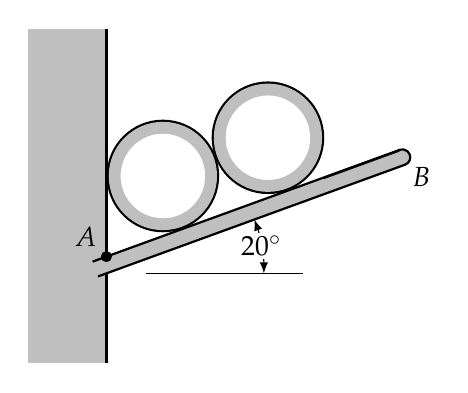
\begin{tikzpicture}[scale=\scale]
	\coordinate (A) at (0,0);
	\coordinate (B) at ($ (A)+(20:4) $);
	\coordinate (AA) at ($ (A)+(0, 0.1067) $);
	\coordinate (C) at ($ (A)+(0, 0.1067)+ (55:1.25) $);
	\coordinate (D) at ($ (C)+(20:1.42) $);

	
	\fill[gray!50] ($ (A)+(0,3) $) rectangle +(-1,-4.25);
	\draw[thick] ($ (A)+(0,3) $) --($ (A)+(0,-1.25) $);

	\draw[line width=0.2cm, gray!50, line cap=round] ($ (A)+(200:0.15) $) -- (B);

	% \Meme{A}{B}{SteelBlue3}{SteelBlue3}{SteelBlue3}{0.3}{0}{0}
	\draw[thick] ($ (A)+(110:0.1)+(200:0.15) $)--+(20:4.15);
	\draw[thick] ($ (A)+(-70:0.1)+(200:0.15) $)--+(20:4.15)arc(-70:130:0.1)--+(200:1);

	\fill (AA)circle(2pt)node[above left] {$ A $};
	\node[below right] at  (B) {$ B $};

	\draw[line width= 0.15cm] (C) circle (0.64cm);
	\draw[line width= 0.15cm,gray!50] (C) circle (0.6125cm);
	\draw[line width= 0.15cm] (D) circle (0.64cm);
	\draw[line width= 0.15cm,gray!50] (D) circle (0.6125cm);

	\draw ($ (A)-(0,0.1067)+(0.5,0) $) -- +(2,0);
	\draw[latex-latex] ($ (A)-(0,0.1067)+(2,0) $) arc(0:20:2)node[midway, fill=white, inner sep=0.4mm]{$ 20\deg $};


\end{tikzpicture}

  }
\end{textblock*}


\begin{textblock*}{4in}(1in, 3.25in)
  \centering
  \large
    The weight of each pipe bearing on $AB$:
    $$ W=78.5\,\text{kg/m}\x 9.81\,\mathsf{m/s^2}\x 10\,\text{m}/3=2.5670\,\text{kN} $$    
\end{textblock*}

\begin{textblock*}{6.75in}(1in, 4in)
  \centering
  \large
  Add some labels, find some distances:\parm
  \mini[0.35]{
    \tikz{%color
      \coordinate (A) at (0,0);
      \coordinate (B) at ($ (A)+(20:4) $);
      \coordinate (D) at ($ (A)+(0, 0.1067)+ (55:1.25) $);
      \coordinate (C) at ($ (D)+(20:1.42) $);
      \coordinate (E) at ($ (D)!0.5!(C)+(110:.625) $);
      \coordinate (F) at ($ (C)+(-70:.64) $);
      \coordinate (G) at ($ (D)+(-70:.64) $);
      \coordinate (H) at ($ (D)+(180:.64) $);
      \draw[thick] ($ (A)+(0,2.5) $) --($ (A)+(0,-0.5) $);
      \draw[line width=0.2cm, gray!50, line cap=round] ($ (A)+(200:0.15) $) -- (B);
      \draw[line width= 0.15cm] (C) circle (0.64cm);
      \draw[line width= 0.15cm,gray!50] (C) circle (0.6125cm);
      \draw[line width= 0.15cm] (D) circle (0.64cm);
      \draw[line width= 0.15cm,gray!50] (D) circle (0.6125cm);
      \node[above, xshift=-2mm] at (A) {$ A $};
      \node[right] at (B) {$ B $};
      \node at (C) {$ C $};
      \node at (D) {$ D $};
      \node at (E) {$ E $};
      \node at ($ (F)+(-70:0.325) $) {$ F $};
      \node at ($ (G)+(-70:0.325) $) {$ G $};
      \node at ($ (H)+(-180:0.325) $) {$ H $};
    }
  }
  \mini[0.3]{
    \tikz{%color
      \coordinate (A) at (0,0);
      \coordinate (B) at ($ (A)+(20:8) $);
      \coordinate (D) at ($ (A)+(55:2.5) $);
      \coordinate (G) at ($ (D)+(-70:1.425) $);
      \coordinate (H) at ($ (D)+(180:1.425) $);

      \draw (A)--(D);
      \draw[thick] (D) circle (1.4cm);
      \draw (A)--($ (A)+(20:4 )$);
      \draw (A)--($ (A)!1.5!(H) $);
      \draw (D)--(G);
      \draw (D)--(H);
      \node[above] at (D) {$ D $};
      \node[left] at (H) {$ H $};
      \node[below] at (G) {$ G $};
      \node[below] at (A) {$ A $};
      \draw ($ (G)+(110:0.5) $)--++(20:0.5)--+(-70:0.5);
    }
  }
  \mini[0.3]{ 
    \begin{align*}
      \angle HAD &= \angle GAD = 35\deg \\
      \angle GAD &= 55\deg \\
      \frac{AG}{GD} &= \tan 55\deg \\
      AG &= \frac{508\,\text{mm}}{2}\tan 55\deg \\
       &=362.75\,\text{mm} \\
      GF &= CD = 508\,\text{mm}
    \end{align*}
  }
  \parb\centering
  {\bf Forces acting upon the upper (rightmost) pipe, $\bm C$}:\parb
  \mini[0.35]{    
      \centering
      \tikz{%color
        \coordinate (O) at (0,0);
        \coordinate (B) at ($ (A)+(20:4) $);
        % \coordinate (D) at ($ (A)+(0, 0.1067)+ (55:1.25) $);
        \coordinate (C) at ($ (D)+(20:1.42) $);
        \node[above] at (C) {$ C $};
        \draw[line width= 0.15cm] (C) circle (0.64cm);
        \draw[line width= 0.15cm,gray!50] (C) circle (0.6125cm);
        \draw[very thick, -latex] (C)--+(0,-1.5)node[below left]{$ 2.5670\,\text{kN} $};
        \draw[very thick, latex-] ($ (C)+(210:0.64) $) --+(210:1.5)node[left]{$ R_E $};
        \draw[very thick, latex-] ($ (C)+(-70:0.64) $) --+(-70:1.5)node[right]{$ R_F $};
      } \parb
      \tikz{%color
        \coordinate (C) at (0,0);
        \draw[very thick, -latex] (C)--+(0,-1.75)node[below]{$ 2.5670\,\text{kN} $};
        \draw[very thick, -latex] (C)--+(110:1.75)node[left]{$ R_F $};
        \draw[very thick, -latex] (C)--+(20:1.75)node[below right]{$ R_E $};
        \draw[latex-latex] ($ (C)+(0,-1.25) $)arc(-90:20:1.25) node[midway, fill=white] {$ 110\deg $};
        \draw[latex-latex] ($ (C)+(110:1.25) $)arc(110:270:1.25) node[midway, fill=white] {$ 160\deg $};
        \node[above,xshift=1mm] at (C) {$ C $};
      }
     
  }
  \hfill
   \mini[0.55]{      
        This is now a simple concurrent forces problem, solved with simultaneous equations. Notice, however, that the direction of $R_F$ is perpendicular to the direction of $R_E$. \parb 
        If we choose axes $x'$ and $y'$, rotated $20\deg$ in the counter clockwise direction around $C$, then the direction of $R_E$ is the $x'$-axis and the direction of $R_F$ is the $y'$-axis. Now we can solve without simultaneous equations.\parb
        (Why bother complicating things? This will become a useful technique towards the end of the module and it's easy to introduce here.)
        \begin{align*}
          \Sigma F_{x'} &= R_E-2.5670\,\text{kN}\cd\cos 70\deg =0 \\
          \Ra R_E &= 0.87800\,\text{kN}\\\\
          \Sigma F_{y'} &= R_F-2.5670\,\text{kN}\cd\cos 20\deg =0 \\
          \Ra R_F &= 2.4122\,\text{kN}\\
        \end{align*}
        \vspace{-1cm}
      
    }
    \end{textblock*}

%%%%%%%%%%%%%%%%%%%%%%%%%%%%%%%%%%%%%%%%%%%%%%%%%%%%%%%%%%%%%%%%%%%%%%%%%%%%%%%%%%%%%%%%%%%%%%%%%%%%
% page 2
%%%%%%%%%%%%%%%%%%%%%%%%%%%%%%%%%%%%%%%%%%%%%%%%%%%%%%%%%%%%%%%%%%%%%%%%%%%%%%%%%%%%%%%%%%%%%%%%%%%%
~\newpage

\begin{textblock*}{6.75in}(1in, 0.5in)
  \large\centering      
    {\bf Forces acting upon the lower (leftmost) pipe, $\bm D$:}
    \parb ~\parb
    \mini[0.35]{
      \centering
      \tikz{%color
        \coordinate (D) at (0,0);
        \node[above] at (D) {$ D $};
        \draw[line width= 0.15cm] (D) circle (0.64cm);
        \draw[line width= 0.15cm,gray!50] (D) circle (0.6125cm);
        \draw[very thick, -latex] (C)--+(0,-1.5)node[below left]{$ 2.5670\,\text{kN} $};
        \draw[very thick, latex-] ($ (C)+(20:0.64) $) --+(20:1.5)node[above]{$ 0.87800\,\text{kN} $};
        \draw[very thick, latex-] ($ (C)+(180:0.64) $) --+(180:1.5)node[left]{$ R_H $};
        \draw[very thick, latex-] ($ (C)+(-70:0.64) $) --+(-70:1.5)node[right]{$ R_G $};
      }
      \parb
       \tikz{%color
        \coordinate (D) at (0,0);
        \draw[very thick, -latex] (D)--+(0,-1.75)node[below]{$ 2.5670\,\text{kN} $};
        \draw[very thick, -latex] (D)--+(110:1.75)node[left]{$ R_G $};
        \draw[very thick, -latex] (D)--+(200:1.75)node[left]{$ 0.87800\,\text{kN} $};
        \draw[very thick, -latex] (D)--+(0:1.75)node[right]{$ R_H $};
        \draw[latex-latex] ($ (D)+(270:1.25) $)arc(270:200:1.25) node[midway, fill=white, inner sep=1mm] {$ 70\deg $};
        \draw[latex-latex] ($ (D)+(0:1.25) $)arc(0:110:1.25) node[midway, fill=white] {$ 110\deg $};
        \node[xshift=-4mm, yshift=2mm] at (D) {$ D $};
        \draw ($ (D)+(0.325,0) $)--++(0,-0.325)--+(-0.325,0);
      }
    }    
    \hfill
    \mini[0.55]{      
        \large
        \begin{align*}          
          \Sigma F_{y} &= R_G\cd\cos 20\deg -2.5670\,\text{kN}-0.87800\,\text{kN}\cd\cos 70\deg\\ &=0 \\
          \Ra R_G &= \frac{2.5670\,\text{kN}+0.87800\,\text{kN}\cd\cos 70\deg}{\cos 20\deg} \\
          \Ra R_G &= 3.0513\,\text{kN}\\
        \end{align*}
        \vspace{-1cm}      
    }
    \parb 
    % A quick check for calculations so far using the vertical components on the two pipes.\parm $ \Sigma F_y = 2.4122\,\text{kN}\cd\cos 20\deg + 3.0513\,\text{kN}\cd\cos 20\deg - 2\x 2.5670\,\text{kN} = 0.000010634\,\text{kN}\qquad  \text{\LARGE\checkmark} $
    % \parb\vspace{1cm}
    \def\scale{1.75}
    \tikz[scale=\scale]{%color
      \coordinate (A) at (0,0);
      \coordinate (B) at ($ (A)+(20:4) $);
      \coordinate (D) at ($ (A)+(0, 0.1067)+ (55:1.25) $);
      % \coordinate (C) at ($ (D)+(20:1.42) $);
      % \coordinate (E) at ($ (D)!0.5!(C)+(110:.625) $);
      \coordinate (F) at ($ (A)+(20:1) $);
      \coordinate (G) at ($ (A)+(20:2.5) $);
     
      \draw[line width=0.35cm, gray!50, line cap=round] ($ (A)+(200:0.15) $) -- (B);
     
      % \node[above, xshift=-2mm] at (A) {$ A $};
      \node[above right] at (B) {$ B $};      
      \node at ($ (F)+(-70:0.125) $) {$ F $};
      \node at ($ (G)+(-70:0.125) $) {$ G $};
      \node[xshift=0.25cm, yshift=-0.8cm] at (A) {$ M $};

      \fill (A) circle (1.5pt) node[xshift=-3mm]{$A $};
      \Couple{A}{black}{0.325}{0.625}
      \draw[ultra thick, -latex] (A)--+(0.75,0)node[below]{$ R_{Ax}$};
      \draw[ultra thick, -latex] (A)--+(0,0.75)node[left]{$ R_{Ay}$};
      \draw[ultra thick, latex-] (G)--+(110:1)node[left]{$3.0513\,\text{kN}$};
      \draw[ultra thick, latex-] (F)--+(110:1)node[left]{$2.4122\,\text{kN}$};

      \coordinate (AA) at ($ (A)+(-70:0.75) $);
      \coordinate (FF) at ($ (F)+(-70:0.75) $);
      \coordinate (GG) at ($ (G)+(-70:0.75) $);
      \draw[thin, gray] (AA)--+(-70:0.5);
      \draw[thin, gray] (FF)--+(-70:0.5);
      \draw[thin, gray] (GG)--+(-70:0.5);
      \draw[thin, gray] ($ (A)+(0:0.875) $)--+(0:1.25);
      \draw[thin] ($ (A)+(20:0.5) $)--+(20:2.5);

      \draw[latex-latex]  ($ (AA)+(-70:0.25) $) -- ($ (FF)+(-70:0.25) $) node[fill=white, midway, rotate=-45] {$ 362.75\,\text{mm}$};
      \draw[latex-latex]  ($ (FF)+(-70:0.25) $) -- ($ (GG)+(-70:0.25) $) node[fill=white, midway,sloped] {$ 508\,\text{mm}$};
      \draw[latex-latex]  ($ (A)+(-0:1.75) $) arc(0:20:1.75) node[midway, fill=white, inner sep=1mm] {$ 20\deg $};

      \draw (F)--++(110:0.2)--++(20:0.2)--+(-70:0.2);
      \draw (G)--++(110:0.2)--++(20:0.2)--+(-70:0.2);
    }

    \begin{align*}
      \Sigma M_A &= M-2.4122\,\text{kN}\cd 362.75\,\text{mm} -3.0513\,\text{kN}\cd 870.75\,\text{mm}=0 \Ra M = 3531.9\,\mathsf{kN\cd mm} = 3.5319\,\mathsf{kN\cd m} \\[0.25em]
      \Sigma F_x &= R_{Ax}+2.4122\,\text{kN}\cd\sin 20\deg +3.0513\,\text{kN}\cd\sin 20\deg=0 \Ra R_{Ax} = -1.8686\,\text{kN} \\[0.25em]
      \Sigma F_x &= R_{Ay}-2.4122\,\text{kN}\cd\cos 20\deg -3.0513\,\text{kN}\cd\cos 20\deg=0 \Ra R_{Ay} = 5.1340\,\text{kN}
    \end{align*}
    \mini[0.2]{
      \tikz[scale=0.75]{%color
        \coordinate (O) at (0,0);
        \draw[-latex, thick] (O) -- +(-1.86,0)node[below]{1.8686\,\text{kN}};
        \draw[-latex, thick] (O) -- +(0,5)node[above]{5.1340\,\text{kN}};
        \draw[-latex, ultra thick] (O) -- +(-1.86,5)node[left]{$ R_A $};
        \node at (-0.5,0.35){$ \theta $};
      }
    }
    \hfill
    \mini[0.75]{
      \begin{align*}
        R_A &= \sqrt{(1.8686\,\text{kN})^2+(5.1340\,\text{kN})^2} = 5.4635\,\text{kN}\\[0.25em]
        \theta &= \tan^{-1}\left[\frac{5.1340\,\text{kN}}{1.8686\,\text{kN}}\right] = 70\deg
      \end{align*}
      \parb
      The reaction at $A$ is $5.46\,\text{kN}$ at $110\deg$ counter-clockwise from the positive $x$-axis. The reacting moment at $A$ is $3.53\,\mathsf{kN\cd m}$
    }

\end{textblock*}
     
      
  
 
     
  


  %  \cbox{
  %   \centering 
  %   Forces acting upon the upper (rightmost) pipe, $C$:\parm 
  %   \mini[0.4]{
  %   \tikz{%color
  %     \coordinate (O) at (0,0);
  %     \coordinate (B) at ($ (A)+(20:4) $);
  %     % \coordinate (D) at ($ (A)+(0, 0.1067)+ (55:1.25) $);
	%     \coordinate (C) at ($ (D)+(20:1.42) $);
  %     \node[above] at (C) {$ C $};
  %     \draw[line width= 0.15cm] (C) circle (0.64cm);
	%     \draw[line width= 0.15cm,gray!50] (C) circle (0.6125cm);
  %     \draw[very thick, -latex] (C)--+(0,-1.5)node[below left]{$ 2.5670\,\text{kN} $};
  %     \draw[very thick, latex-] ($ (C)+(210:0.64) $) --+(210:1.5)node[left]{$ R_E $};
  %     \draw[very thick, latex-] ($ (C)+(-70:0.64) $) --+(-70:1.5)node[right]{$ R_F $};
  %   } 
  %   }
  %  }
  % }




~\newpage

\begin{textblock*}{3.5in}(1in, 5.5in)
	\cbox{
		\underbar{\bf Example 2:} Determine the sum of the moments of the forces, acting at $B$ and $C$, about the point $A$. \parm  Also, sum the moments of the forces about the point $B$.
	}
\end{textblock*}
\begin{textblock*}{2.75in}(5.025in, 5.5in)
	\cbox{
		\centering
		\def\scale{0.8}
		% !TEX root = ../../Beamer/statikz/statikz.tex


\tikz[scale=\scale]{
	\small
	\def\hi{0.2}


	\def\extend{0.5}

	\coordinate (A) at (0,0);
	\coordinate (B) at (4,0);
	\coordinate (C) at (4,2);

	\filldraw[fill=Gray!50, draw=black, thick, rounded corners=1mm] ($ (A)+(-1,4) $) -- ++(1,0) -- ++(0,-3.65) -- ($ (B)+(-0.35,0.35) $) -- ($ (C)+(-0.35,0.5) $)  -- ($ (C)+(0.35,0.5) $) -- ($ (B)+(0.35,-0.35) $)-- ($ (A)+(0,-0.35)  $)--++(0,-2)--+(-1,0);

	\draw[ultra thick, -latex, name path=BD] (B) -- +(131:3.75) node[above] {$2.30\,$kN};
	\draw[ultra thick, -latex, line cap=round] (C) -- +(90:1.5) node[above, black] {$2.05\,$kN};
	\draw[ultra thick, -latex, line cap=round] (C) -- +(0:1.75) node[above, black] {$2.84\,$kN};
	\draw ($ (B)-(1.5,0) $) -- ($ (B)-(2.5,0) $);
	\draw ($ (C)+(1,0) $) -- +(1:0);

	\draw[latex-latex] ($ (B)+(131:2)  $) arc (131:180:2);

	\fill[black] (A) circle (2pt) node[left] {$\bm A$};
	\fill[black] (B) circle (2pt) node[below right, outer sep=2mm] {$\bm B$};
	\fill[black] (C) circle (2pt) node[xshift=0.25mm, above right, outer sep=2mm] {$\bm C$};
	\node[fill=white] at ($ (B)+(155:2) $){$49^\circ$};
	\draw ($ (B)+(0.5,0) $) -- +(1,0);
	\draw ($ (B)+(0,-0.5) $) -- +(0,-1);
	\draw[latex-latex] ($ (A)-(0,1) $) -- node[fill=white] {$4.00\,$m} ($ (B)-(0,1) $);
	\draw[latex-latex] ($ (C)+(1,0) $) -- node[fill=white, xshift=0.25cm] {$2.00\,$m} ($ (B)+(1,0) $);

  % \path[name path=AD] (A)--+(41:4);
  % \path[name intersections={of=AD and BD, by={D}}] ;
  % \draw (A)--(D)node[midway, fill=white] {$ d $};
  % \draw ($ (D)+(131:0.325) $) --++(221:0.325)--+(-49:0.325);

}

	}
\end{textblock*}
\begin{textblock*}{3.5in}(1in, 7in)
  \centering
  \tikz[scale=0.875]{%color
    \coordinate (A) at (0,0);
    \coordinate (B) at (4,0);
    \coordinate (C) at (4,2);
    \draw[gray!50, line width=5mm, line cap=round] (A)--(B)--(C);
    \draw[ultra thick, -latex, name path=BD] (B) -- +(131:3.75) node[above] {$2.30\,$kN};
    \draw[ultra thick, -latex, line cap=round] (C) -- +(90:1.5) node[above, black] {$2.05\,$kN};
    \draw[ultra thick, -latex, line cap=round] (C) -- +(0:1.75) node[above, black] {$2.84\,$kN};
    \draw ($ (B)-(1.5,0) $) -- ($ (B)-(2.5,0) $);
    \draw ($ (C)+(1,0) $) -- +(1:0);
	  \draw[latex-latex] ($ (B)+(131:2)  $) arc (131:180:2);
    \fill[black] (A) circle (2pt) node[left, xshift=-0.25cm] {$\bm A$};
    \fill[black] (B) circle (2pt) node[below right, outer sep=2mm] {$\bm B$};
    \fill[black] (C) circle (2pt) node[xshift=0.25mm, above right, outer sep=2mm] {$\bm C$};
    \node[fill=white] at ($ (B)+(155:2) $){$49^\circ$};
    \draw ($ (B)+(0.5,0) $) -- +(1,0);
    \draw ($ (B)+(0,-0.5) $) -- +(0,-1);
    \draw ($ (A)+(0,-0.5) $) -- +(0,-1);
    \draw[latex-latex] ($ (A)-(0,1) $) -- node[fill=white] {$4.00\,$m} ($ (B)-(0,1) $);
    \draw[latex-latex] ($ (C)+(1,0) $) -- node[fill=white, xshift=0.25cm] {$2.00\,$m} ($ (B)+(1,0) $);
      \path[name path=AD] (A)--+(41:4);
  \path[name intersections={of=AD and BD, by={D}}] ;
  \draw (A)--(D)node[midway, fill=white] {$ d $};
  \draw ($ (D)+(131:0.325) $) --++(221:0.325)--+(-49:0.325);
  }
  \large
  \begin{align*}
    \Sigma M_A &= \Sigma F\cd d \\[0.25em]
    &= (2.30\,\text{kN})\cd(4.00\,\text{m})(\sin 49\deg) \\
    &\qquad +(2.05\,\text{kN})\cd(4.00\,\text{m}) \bm - (2.84\,\text{kN})\cd(2.00\,\text{m})\\[0.25em]
    &= 9.4633\,\mathsf{kN\cd m} 
    \approx 9.46 \,\mathsf{kN\cd m} \\\\
    \Sigma M_B &= 0+0-(2.84\,\text{kN})\cd(2.00\,\text{m})=-5.6800\,\mathsf{kN\cd m}
    = -5.68\,\mathsf{kN\cd m}
  \end{align*}
\end{textblock*}

%%%%%%%%%%%%%%%%%%%%%%%%%%%%%%%%%%%%%%%%%%%%%%%%%%%%%%%%%%%%%%%%%%%%%%%%%%%%%%%%%%%%%%%%%%%%%%%%%%%
% page 2
%%%%%%%%%%%%%%%%%%%%%%%%%%%%%%%%%%%%%%%%%%%%%%%%%%%%%%%%%%%%%%%%%%%%%%%%%%%%%%%%%%%%%%%%%%%%%%%%%%%
~\newpage


\end{document}